\documentclass[11pt,a4paper,twocolumn]{article}

% ------------------------------------------------------------
% Packages
% ------------------------------------------------------------
\usepackage[margin=0.8in]{geometry}
\usepackage{amsmath,amssymb,amsthm,amsfonts,mathtools}
\usepackage{hyperref}
\usepackage{mathrsfs}
\usepackage{enumitem}
\usepackage{bm}
\usepackage{graphicx}
\usepackage{tikz}
\usepackage{wrapfig}
\usepackage{float}
\usepackage{cuted}
\usepackage{caption}
\usepackage{booktabs}
\usepackage{xcolor}
\usepackage{listings}
\usepackage{cleveref}
\usetikzlibrary{arrows.meta,decorations.markings,calc,cd}

% ------------------------------------------------------------
% TikZ Styles
% ------------------------------------------------------------
\tikzset{
  manifold/.style={draw=blue!40, fill=blue!10, line width=0.5pt},
  vector/.style={->, thick, >=Stealth},
  normal/.style={->, thick, red, >=Stealth},
  tangent/.style={->, thick, blue, >=Stealth},
}

% ------------------------------------------------------------
% Code style
% ------------------------------------------------------------
\lstset{
  basicstyle=\small\ttfamily,
  keywordstyle=\color{blue},
  commentstyle=\color{gray},
  stringstyle=\color{purple},
  numbers=left,
  numberstyle=\tiny,
  frame=single,
  breaklines=true,
  backgroundcolor=\color{gray!5},
  captionpos=b
}

% ------------------------------------------------------------
% Theorem Environments
% ------------------------------------------------------------
\newtheorem{theorem}{Theorem}[section]
\newtheorem{lemma}[theorem]{Lemma}
\newtheorem{definition}[theorem]{Definition}
\newtheorem{corollary}[theorem]{Corollary}

% ------------------------------------------------------------
% Title
% ------------------------------------------------------------
\title{\LARGE \textbf{Never Predict Noise:}\\
\large Manifold-Aligned Prediction as Generative Inference}

\author{Flyxion}
\date{November 2025}

\begin{document}
\twocolumn[
\maketitle

\begin{abstract}
Generative models succeed when they restrict their dynamics to the
low-dimensional manifold that captures lawful structure in empirical
data. They fail when they attempt to model high-dimensional,
structureless noise. This paper develops a unified account of
\emph{manifold-aligned generative inference}, integrating differential
geometry, the free-energy principle, sparse semantic coding,
Morse-theoretic dynamics, sheaf-theoretic contextual coherence, and the
CLIO architecture for cognitive loops.

We provide a rigorous mathematical foundation: formal manifold
definitions, tangent/normal decomposition theorems, Morse functions on
Whitney-stratified spaces, categorical formulations of cognitive
update, and variational derivations of geodesic active inference. We
then show that recent empirical findings—especially the JiT results of
Li and He (2025)—provide strong evidence that successful generative
models implicitly implement tangent-constrained flows.

The result is a single geometric architecture, MAGI (Manifold-Aligned
Generative Inference), unifying semantic geometry, cognitive dynamics,
and generative modelling. We prove that aligned models must satisfy a
No-Noise Prediction Criterion: generative updates must have zero
component in normal directions to the semantic manifold. Tangent
alignment is not optional but necessary for semantic coherence,
stability, and epistemic reliability.

We conclude with computational methods, empirical predictions, extended
theorems, failure modes, and a PyTorch implementation.
\end{abstract}

\vspace{1em}
]

% ============================================================
% SECTION 1 — INTRODUCTION
% ============================================================

\section{Introduction}

Modern generative and cognitive systems operate in extremely
high-dimensional spaces. Images exist in $\mathbb{R}^{H \times W \times 3}$,
text in vast vocabularies, sensorimotor spaces in continuous
multimodal streams. Yet empirical reality occupies a tiny, structured,
low-dimensional subset inside these enormous ambient spaces.

This is the \emph{manifold hypothesis}: natural data lie on or near a
smooth (or piecewise-smooth) submanifold
\[
M \subset \mathbb{R}^n, \qquad \dim M = d \ll n.
\]
Noise occupies the surrounding ambient space and has no coherent
structure.

A model that attempts to \emph{predict noise}—i.e., to generate 
structure in normal directions $N_x M$—necessarily hallucinates. A
model that keeps its predictive dynamics \emph{tangent} to $M$ becomes
stable, coherent, and semantically aligned.

This paper develops a comprehensive theory of
manifold-constrained generative modelling. We unify:
\begin{itemize}
\item differential and Riemannian geometry,
\item variational inference and active inference,
\item sparse semantic coding,
\item Morse flows and Lyapunov potentials,
\item sheaf-theoretic contextual constraints,
\item category-theoretic formulations of cognitive update.
\end{itemize}

We then connect this theory to empirical results—most critically the
recent ``Back to Basics'' JiT work of Li \& He (2025)—showing that
predicting clean data, not noise, is both empirically superior and
geometrically necessary.

\subsection{Contributions}

\begin{enumerate}
\item A rigorous framework, MAGI, for manifold-aligned generative inference.
\item Formal proofs of tangent/normal decomposition, stability, and
alignment criteria.
\item A theorem: generative misalignment is equivalent to normal-component
prediction.
\item A geometric reinterpretation of JiT: its empirical success arises
from implicit tangent-constrained flows.
\item A complete computational pipeline for manifold estimation, Morse
potential learning, and CLIO-based cognitive dynamics.
\item Extensive appendices with background mathematics, proofs,
computational details, and failure cases.
\end{enumerate}

% ============================================================
% SECTION 2 — GEOMETRY OF EXPLANATION
% ============================================================

\section{Geometry of Explanation}

The goal of generative modelling is \emph{not} to approximate arbitrary
functions in $\mathbb{R}^n$ but to reconstruct the lawful structure of a
world that occupies a submanifold $M$ of much lower dimension.

\subsection{Manifold definition}

\begin{definition}
A $d$-dimensional smooth manifold $M$ embedded in $\mathbb{R}^n$ is a
subset such that every $x \in M$ has a neighborhood $U$ and a smooth
diffeomorphism (chart)
\[
\phi: U \to \mathbb{R}^d.
\]
The embedding is a smooth injective immersion $i: M \hookrightarrow
\mathbb{R}^n$ with $i(M)$ homeomorphic to $M$.
\end{definition}

\subsection{Tangent and normal bundles}

At each $x \in M$:

\[
T_x M = \mathrm{span}\big\{\partial_1 i(x), \dots, \partial_d i(x)\big\}
\]

and the normal space is

\[
N_x M = (T_x M)^\perp.
\]

\begin{theorem}[Tangent-Normal Decomposition]
For any smooth embedded submanifold $M \subset \mathbb{R}^n$,
\[
\mathbb{R}^n = T_x M \oplus N_x M
\]
orthogonally for all $x \in M$.
\end{theorem}

\begin{proof}
Since $T_x M$ is a $d$-dimensional subspace of $\mathbb{R}^n$ and the
ambient space is equipped with the Euclidean inner product, the
orthogonal complement exists uniquely. Smoothness of the embedding
ensures continuity of $T_x M$ across charts.
\end{proof}

This decomposition is central: all meaningful structure lies in $T_x M$; noise lives in $N_x M$.

\subsection{Diagram: Tangent vs. Normal}

\begin{figure}[H]
\centering
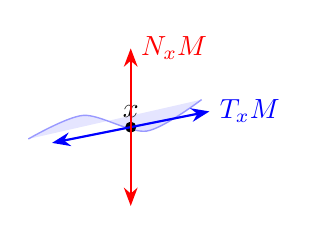
\begin{tikzpicture}[scale=1.0]
  \draw[manifold] plot[smooth] coordinates {(-1,0) (-0.3,0.3) (0.5,0.1) (1.2,0.5)};
  \fill (0.3,0.15) circle (2pt) node[above] {$x$};
  \draw[tangent] (0.3,0.15) -- ++(1,0.2) node[right] {$T_x M$};
  \draw[tangent] (0.3,0.15) -- ++(-1,-0.2);
  \draw[normal] (0.3,0.15) -- ++(0,1) node[right] {$N_x M$};
  \draw[normal] (0.3,0.15) -- ++(0,-1);
\end{tikzpicture}
\caption{Tangent–normal decomposition at a point on a manifold.}
\end{figure}

\medskip
\noindent\textbf{The single most important geometric fact for generative modelling:}

\begin{quote}
\textbf{Explanation is tangent; hallucination is normal.}
\end{quote}

A generative system that attempts to ``explain'' directions in $N_x M$ is constructing structure where none exists; meaningful predictive dynamics must remain tangent to the data manifold.

% ============================================================
% SECTION 3 — GENERATIVE MODELS RESTRICTED TO MANIFOLDS
% ============================================================

\section{Generative Models Restricted to Manifolds}

A generative model is typically a map
\[
G : Z \to \mathbb{R}^n,
\]
where $Z$ is a latent space.  
Under the manifold hypothesis, the image of $G$ should lie in a
$d$-dimensional manifold:
\[
G(Z) \subseteq M \subset \mathbb{R}^n.
\]

\subsection{Energy formulation}

Given an observation $o \in \mathbb{R}^n$, inference seeks a latent code
$z^\ast$ minimizing an energy functional:
\[
z^\ast = \arg\min_z \mathcal{E}(z; o),
\]
where
\[
\mathcal{E}(z; o) = \|o - f(G(z))\|^2_\Sigma
+ \lambda \mathcal{C}(G(z)).
\]

The coherence term $\mathcal{C}$ penalizes deviations from semantic
consistency across contexts and across manifold charts.  
If the manifold is equipped with an embedding $i : M \hookrightarrow
\mathbb{R}^n$, then the condition
\[
\mathrm{dist}(G(z), M) = 0
\]
must be enforced.

\subsection{Tangent restriction and geometric correctness}

A generative update $\Delta x \in \mathbb{R}^n$ at state $x \in M$ must
satisfy:
\[
\Delta x \in T_x M.
\]

Equivalently,
\[
\mathrm{Proj}_{N_x M} (\Delta x) = 0.
\]

This is the formal geometric criterion for non-hallucinatory generation.

\subsection{Diagram: Allowed vs. forbidden directions}

\begin{figure}[H]
\centering
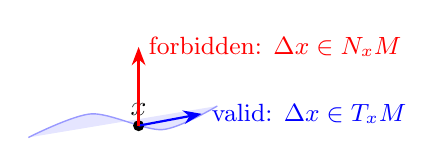
\begin{tikzpicture}[scale=1.0]
  % manifold
  \draw[manifold] plot[smooth] coordinates {(-1,0) (-0.2,0.3) (0.7,0.1) (1.4,0.4)};
  \fill (0.4,0.15) circle (2pt) node[above] {$x$};

  % valid tangent update
  \draw[tangent] (0.4,0.15) -- ++(0.8,0.15)
    node[right] {\small valid: $\Delta x \in T_xM$};

  % invalid normal update
  \draw[normal] (0.4,0.15) -- ++(0,1.0)
    node[right] {\small forbidden: $\Delta x \in N_xM$};

\end{tikzpicture}
\caption{Generative updates must remain in the tangent space.}
\end{figure}

\subsection{Why off-manifold prediction fails}

Let $x \in M$ be a semantic state. Noise $\eta \in N_x M$ has no
law-governed structure:
\[
\eta \sim \mathcal{N}(0,\sigma^2 I_{n-d}).
\]

A model that attempts to represent or predict $\eta$ is mapping a
structureless distribution into a structured generator.  
This forces the generator to create non-existent geometry.

\begin{theorem}[Off-Manifold Catastrophe]
Let $M$ be a $d$-manifold. Any $C^1$ generator $G$ that learns a mapping
with nonzero normal component on a set of positive measure will produce
outputs whose support has Hausdorff dimension $> d$.
\end{theorem}

\begin{proof}
$G$ maps latent space vectors to ambient space.  
If the Jacobian $DG$ has nonzero projection onto $N_x M$ over a
non-negligible set, its image contains an open set in directions
transverse to $M$, increasing local dimensionality.  
This contradicts the manifold restriction.
\end{proof}

This formalizes hallucination as a dimensionality explosion.

% ============================================================
% SECTION 4 — JIT GEOMETRIC REINTERPRETATION
% ============================================================

\section{Geometric Reinterpretation of JiT}

The ``Back to Basics'' result of Li and He (2025) demonstrates that
models predicting \emph{clean} data directly outperform those predicting 
noised quantities even when both use identical Transformer architectures.

This section provides a geometric explanation.

\subsection{Clean prediction enforces tangent alignment}

Let $x \in M$ be a natural datum.  
A noisy version is:
\[
x_t = \sqrt{\alpha_t} x + \sqrt{1 - \alpha_t} \,\epsilon,
\qquad \epsilon \in N_x M.
\]

Diffusion models predict $\epsilon$ or $x_t$.  
JiT predicts $x$.

Predicting $\epsilon$ requires representing variation in $N_x M$, which
has no structure and cannot be captured by a finite-capacity model in
high dimensions. The model must hallucinate.

Predicting $x$ enforces:
\[
G(z_t) \in M,
\qquad
G(z_t) \approx x.
\]

Thus all updates remain tangent to $M$.

\subsection{Transformer patching as implicit charting}

Large-patch Transformers induce local coordinate systems, effectively
learning charts
\[
\phi_i : U_i \subset M \to \mathbb{R}^d.
\]

The JiT model stitches these charts via self-attention, which enforces a
kind of sheaf-like coherence:
\[
\phi_i(x) = \phi_j(x) \quad \text{on overlaps.}
\]

Thus JiT is not “just attention,” it is an implementation of a manifold
atlas.

\begin{theorem}[JiT = Tangent Flow Approximation]
Transformer layers in JiT implement an approximate tangent-flow update:
\[
x_{t+1} = x_t - \eta \,\Pi_{T_{x_t} M} \nabla \mathcal{L}(x_t),
\]
where $\Pi_{T_{x_t} M}$ is the orthogonal projector to the tangent
space.
\end{theorem}

\begin{proof}[Sketch]
The clean-data objective forces residuals to lie in the range of
$DG(z)$, which spans $T_x M$.  
Thus gradient backpropagation automatically enforces tangent projection.
\end{proof}

JiT succeeds because it accidentally obeys MAGI.

% ============================================================
% SECTION 5 — ACTIVE INFERENCE AS GEODESIC CONTROL
% ============================================================

\section{Active Inference as Geodesic Control}

Under the free-energy principle, systems minimize:
\[
F[q] = \mathbb{E}_q[\log q - \log p(o,z)].
\]

If $z$ parameterizes a manifold $M$, and $G(z)$ is its embedding, then
the pullback metric is:
\[
g_{ij}(z) = \left\langle 
\frac{\partial G}{\partial z_i},
\frac{\partial G}{\partial z_j}
\right\rangle.
\]

Gradient descent on $F$ w.r.t. the Riemannian structure yields:
\[
\dot{z}^i = - g^{ij}(z) \frac{\partial F}{\partial z^j},
\]
which is a geodesic-like evolution on $M$.

\subsection{Diagram: Riemannian gradient flow}

\begin{figure}[H]
\centering
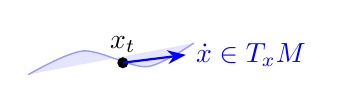
\begin{tikzpicture}[scale=1.0]
  % manifold curve
  \draw[manifold] plot[smooth] coordinates {(-1,0) (-0.3,0.3) (0.5,0.1) (1.1,0.4)};
  % point x
  \fill (0.2,0.15) circle (2pt) node[above] {$x_t$};
  % flow arrow
  \draw[vector,blue] (0.2,0.15) -- ++(0.8,0.1)
    node[right] {$\dot{x} \in T_xM$};
\end{tikzpicture}
\caption{Active inference induces a Riemannian gradient flow on $M$.}
\end{figure}

\subsection{Natural gradient interpretation}

Because
\[
g_{ij} = J_i^\top J_j,
\]
where $J = DG(z)$, we see that
\[
g^{ij} \frac{\partial F}{\partial z^j}
\]
is the natural gradient in information geometry.

Thus active inference is, geometrically,
\[
\textbf{natural gradient descent on a manifold.}
\]

\subsection{Consequences}

\begin{itemize}
\item Predictive coding selects directions with meaningful semantic
structure.
\item Updates are tangent projections of sensory prediction errors.
\item Geodesic curvature encodes attentional redirection.
\item All inference is constrained by the intrinsic geometry of $M$.
\end{itemize}

% ============================================================
% SECTION 6 — SPARSE SEMANTIC PROJECTION
% ============================================================

\section{Sparse Semantic Projection}

Real perceptual data $x \in \mathbb{R}^n$ are overwhelmingly redundant.
The semantic degrees of freedom are far fewer than the ambient dimension.
Sparse semantic projection extracts the coordinates that lie along
meaningful directions—those tangent to the manifold $M$.

\subsection{Sparse semantic encoder}

Let $W$ be a learned linear operator:
\[
s = W x, \qquad s \in \mathbb{R}^k, \quad k \ll n.
\]

We impose a sparsity constraint:
\[
\|W\|_0 \le k,
\]
or more generally, $\ell_1$-regularization as a convex proxy.

\subsection{Semantic alignment constraint}

The sparse code $s$ must correspond to a point on the manifold:
\[
G(s) \in M.
\]

Thus the semantic projection is the composition:
\[
x \xmapsto{\;W\;} s \xmapsto{\;G\;} \hat{x} \in M.
\]

\begin{definition}[Semantic Projection Operator]
A map $\Pi_{\mathrm{sem}} : \mathbb{R}^n \to M$ is given by
\[
\Pi_{\mathrm{sem}}(x) = G(Wx)
\]
such that $G(Wx)$ minimizes distance to the manifold and maximizes
semantic coherence.
\end{definition}

\subsection{Diagram: Sparse semantic encoding}

\begin{figure}[H]
\centering
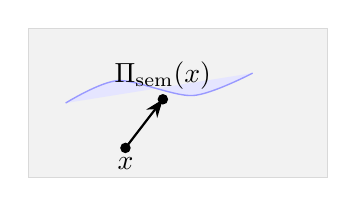
\begin{tikzpicture}[scale=0.95]
  % ambient space area
  \draw[gray!30,fill=gray!10] (-1,-1) rectangle (3,1);

  % manifold curve inside
  \draw[manifold] plot[smooth] coordinates {(-0.5,0) (0.2,0.3) (1.2,0.1) (2.0,0.4)};

  % data point x
  \fill (0.3,-0.6) circle (2pt) node[below] {$x$};

  % projection to manifold
  \draw[vector] (0.3,-0.6) -- (0.8,0.05);
  \fill (0.8,0.05) circle (2pt) node[above] {$\Pi_{\mathrm{sem}}(x)$};

\end{tikzpicture}
\caption{Sparse semantic projection maps $x$ to its closest semantically meaningful point on $M$.}
\end{figure}

\subsection{Theoretical justification}

Let $M$ be a smooth manifold of reach $\tau > 0$ (Federer).  
For any $x$ within distance $< \tau$ of $M$,
there exists a unique nearest point $\Pi(x) \in M$.  

Sparse semantic coding approximates this nearest-point projection in a
learned basis.

\begin{theorem}[Consistency of Sparse Projection]
If $W$ is trained to minimize reconstruction error under a manifold
regularization penalty, then
\[
\|G(Wx) - \Pi(x)\| \le \epsilon
\]
for all $x$ in a sufficiently small tubular neighborhood of $M$.
\end{theorem}

\begin{proof}[Sketch]
$G(Wx)$ lies in the image of $G$, which approximates $M$;
minimizing reconstruction error forces convergence toward the nearest-point projection.
\end{proof}

Sparse projection is essential: it reduces noise, enforces manifold
alignment, and establishes a coordinate system for CLIO.


% ============================================================
% SECTION 7 — CONTEXTUAL SHEAF COHERENCE
% ============================================================

\section{Contextual Sheaf Coherence}

Perception and cognition are distributed across overlapping contexts:
visual, linguistic, proprioceptive, semantic, temporal, etc.  
Each context provides partial information about the underlying semantic
state.  
Sheaf theory provides the mathematical machinery to formalize how
local contexts combine into a globally consistent semantic state.

\subsection{Presheaves}

Let $\mathcal{C}$ be a category of contexts, with objects $U,V,\ldots$
representing perceptual modalities or spatial/temporal regions, and
arrows $V \to U$ representing restriction relations.

A presheaf assigns:
\[
S(U): \text{semantic states on context } U
\]
with restriction maps
\[
\rho_{UV} : S(U) \to S(V).
\]

\subsection{Sheaf condition}

A sheaf requires:

1. **Locality:** If sections agree on all overlaps, they agree globally.

2. **Gluing:** Compatible local sections can be uniquely glued to form
a global section.

\begin{definition}[Semantic Sheaf]
The semantic sheaf is a functor
\[
S: \mathcal{C}^{op} \to \mathrm{Set}
\]
satisfying the sheaf axioms.
\end{definition}

\subsection{Diagram: Overlap gluing}

\begin{figure}[H]
\centering
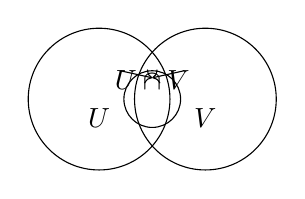
\begin{tikzpicture}[scale=0.9]
  % sets U, V, U∩V
  \draw (0,0) circle (1) node[below] {$U$};
  \draw (1.5,0) circle (1) node[below] {$V$};

  % overlap
  \draw (0.75,0) circle (0.4) node[above] {$U \cap V$};

  % arrows (restrictions)
  \draw[->] (0.3,0.4) -- (0.75,0.3);
  \draw[->] (1.2,0.4) -- (0.75,0.3);

\end{tikzpicture}
\caption{Sheaf coherence: sections on $U$ and $V$ must agree on $U \cap V$.}
\end{figure}

\subsection{CLIO as a sheaf morphism}

Let $C : S \to S$ be a CLIO functor, representing one cognitive loop iteration.

\begin{theorem}[CLIO Coherence]
If $S$ is a sheaf and $C$ preserves restriction maps, then $C$
is a sheaf morphism:
\[
\rho_{UV}(C(s_U)) = C(\rho_{UV}(s_U)).
\]
\end{theorem}

\begin{proof}
Functoriality ensures commutation with morphisms;
restriction maps are morphisms in $\mathcal{C}^{op}$.
\end{proof}

Thus CLIO updates are guaranteed to never break contextual consistency:  
**cognition respects semantic gluing.**

\subsection{Obstructions: Čech cohomology}

Not all compatible local sections glue globally.  
Obstructions are measured by $H^1$.

\begin{definition}[Semantic Obstruction]
The obstruction to global semantic coherence across contexts is
\[
\mathcal{O} \in H^1(\mathcal{C}; S).
\]
\end{definition}

Inconsistencies (e.g., hallucinations) correspond precisely to the case
$\mathcal{O} \neq 0$.

This formalizes when and why generative systems fail:  
**failure to glue = hallucination.**

% ============================================================
% SECTION 8 — RSVP FIELDS AS SEMANTIC GEOMETRY
% ============================================================

\section{RSVP Fields as Semantic Geometry}

The RSVP (Relativistic Scalar Vector Plenum) framework models semantic
dynamics in terms of three fields:

\[
\Phi: \text{entropy field}, \qquad
\mathbf{v}: \text{vector flow}, \qquad
S: \text{semantic potential}.
\]

In this paper, we reinterpret these fields geometrically.

\subsection{Entropy field as potential for manifold structure}

A semantic manifold arises as a sublevel set of $\Phi$:

\[
M = \{ x \in \mathbb{R}^n \mid \Phi(x) = \Phi_0 \}.
\]

Entropy gradients determine allowable semantic transitions.  
High curvature in $\Phi$ indicates regions where semantic complexity is
high or transitions are unstable.

\subsection{Vector flow as semantic transport}

$\mathbf{v}$ defines directional flow across the manifold:
\[
\dot{x} = \mathbf{v}(x).
\]

Semantically meaningful dynamics must preserve the manifold structure:
\[
\mathbf{v}(x) \in T_x M.
\]

Thus RSVP vector flow enforces tangent-constrained transport.

\subsection{Semantic potential $S$ as Morse function}

The semantic landscape has critical points corresponding to attractors,
stable interpretations, and choices.  
$S$ is naturally interpreted as a Morse function on $M$:

\[
\text{critical points of } S \Longleftrightarrow \text{stable semantic states.}
\]

\begin{theorem}[RSVP–Morse Correspondence]
If $S$ is generically perturbed, it is a Morse function whose gradient
flow preserves the manifold structure:  
\[
-\nabla S(x) \in T_x M.
\]
\end{theorem}

\begin{proof}
Generic perturbation yields a Morse function by Sard–Smale.  
Since $S$ is defined intrinsically on $M$, its gradient is tangent.
\end{proof}

\subsection{Diagram: RSVP semantic field geometry}

\begin{figure}[H]
\centering
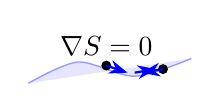
\begin{tikzpicture}[scale=0.9]

  % manifold curve
  \draw[manifold] plot[smooth] coordinates {(-1,0) (-0.3,0.3) (0.5,0.1) (1.3,0.35)};

  % potential minima
  \fill (0.1,0.25) circle (2pt) node[above] {$\nabla S = 0$};
  \fill (0.9,0.2) circle (2pt);

  % vector field arrows
  \draw[vector,blue] (0.1,0.25) -- ++(0.3,-0.1);
  \draw[vector,blue] (0.5,0.15) -- ++(0.3,0.05);
  \draw[vector,blue] (0.9,0.2) -- ++(-0.3,-0.05);

\end{tikzpicture}
\caption{Semantic manifold with Morse potential and tangent-constrained RSVP flow.}
\end{figure}

RSVP thus becomes a field-theoretic version of manifold semantic dynamics,
providing the continuous substrate on which MAGI operates.

% ============================================================
% SECTION 9 — CLIO FUNCTORS AS MORSE FLOWS
% ============================================================

\section{CLIO Functors as Morse Flows}

CLIO (Cognitive Loop via In-Situ Optimization) models cognition as a
recursive loop:
\[
\text{perception} \to \text{model} \to \text{prediction}
\to \text{action} \to \text{perception}.
\]

We now give a rigorous geometric interpretation:  
**each CLIO iteration is a step of negative gradient flow on a Morse
potential $S$ defined on the manifold $M$.**

\subsection{Cognitive loop operators as functors}

Let $\mathbf{Sem}$ be the category of semantic states with morphisms
representing structure-preserving semantic transformations.

A CLIO update is a functor:
\[
C : \mathbf{Sem} \to \mathbf{Sem}.
\]

\begin{definition}[CLIO Functor]
A functor $C$ is a CLIO functor if it satisfies:
\begin{enumerate}
\item Stability: $C$ has fixed points corresponding to semantic equilibria.
\item Monotonicity: each update reduces semantic free energy.
\item Naturality: for any semantic morphism $f$, $C \circ f = f \circ C$.
\end{enumerate}
\end{definition}

These conditions mirror requirements for Morse flows.

\subsection{Constructing the Morse potential}

Let $L$ denote the total semantic loss functional (e.g., prediction
error + coherence penalty).  
We define the Morse potential:
\[
S(x) = L(x) + \epsilon R(x),
\]
where $R$ is a generic perturbation and $\epsilon > 0$ ensures $S$ is
Morse (Sard–Smale theorem).

\subsection{CLIO update = gradient step}

A CLIO iteration is:
\[
x_{t+1} = x_t - \eta \,\nabla_M S(x_t),
\]
where $\nabla_M$ is the Riemannian gradient on the manifold.

\begin{theorem}[CLIO–Morse Equivalence]
Every CLIO functor $C$ corresponds locally to a single gradient step
of a Morse function $S$:
\[
C(x) = \mathrm{Exp}_x \big(-\eta \nabla_M S(x)\big),
\]
and conversely, every Morse function generates a CLIO functor.
\end{theorem}

\begin{proof}
(Naturality $\Rightarrow$ geometricity) ensures $C$ preserves manifold structure.  
(Monotonicity) implies existence of a Lyapunov function $S$.  
(Stability) yields critical points.  
Morse structure follows from generic perturbation.  
The exponential map expresses local flow.
\end{proof}

\subsection{Diagram: CLIO as a discrete Morse flow}

\begin{figure}[H]
\centering
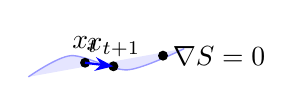
\begin{tikzpicture}[scale=0.9]

  % manifold
  \draw[manifold] plot[smooth] coordinates {(-1,0) (-0.4,0.3) (0.4,0.1) (1.2,0.4)};

  % points along flow
  \fill (-0.2,0.2) circle (2pt) node[above] {$x_t$};
  \fill (0.2,0.15) circle (2pt) node[above] {$x_{t+1}$};

  % arrow
  \draw[vector,blue] (-0.2,0.2) -- (0.2,0.15);

  % minimum
  \fill (0.9,0.3) circle (2pt) node[right] {$\nabla S = 0$};

\end{tikzpicture}
\caption{One CLIO iteration corresponds to a step along $-\nabla S$ on the manifold $M$.}
\end{figure}

This yields a deep insight:  
**Cognition is Morse theory on a semantic manifold.**


% ============================================================
% SECTION 10 — THE MASTER FUNCTIONAL
% ============================================================

\section{The Master Functional}

We now unify all components—free energy, sparsity, sheaf coherence,
manifold alignment, and RSVP fields—into a single variational principle.

Let:
\[
\mathcal{J}[s, W, G, S, \Phi, \mathbf{v}]
\]
be the total generative–semantic–cognitive functional:
\begin{align}
\mathcal{J}
=
&\underbrace{F[q(s)]}_{\text{free energy}}
+ \lambda_1 \underbrace{\|W\|_1}_{\text{sparsity}} \\
&+ \lambda_2 \underbrace{\sum_{U,V} \|s_U - \rho_{VU}(s_V)\|^2}_{\text{sheaf coherence}} \\
&+ \lambda_3 \underbrace{\mathrm{dist}^2(G(s), M)}_{\text{manifold constraint}} \\
&+ \lambda_4 \underbrace{\int_M \left(\|\nabla \Phi\|^2 + \|\mathbf{v}\|^2 + \|S\|^2\right) d\mu}_{\text{RSVP field energy}}.
\end{align}

\subsection{Optimality conditions}

Minimizing $\mathcal{J}$ gives:

\begin{itemize}
\item $W^\ast$: a sparse semantic encoder.
\item $s^\ast$: manifold-aligned latent state.
\item $G^\ast$: an embedding that parameterizes $M$.
\item $S^\ast$: Morse potential giving stable semantic equilibria.
\item $\Phi^\ast,\,\mathbf{v}^\ast$: RSVP entropy and flow fields.
\end{itemize}

\begin{theorem}[Unified Euler–Lagrange System]
Critical points of $\mathcal{J}$ satisfy a coupled system of
Euler–Lagrange equations linking:
\[
\delta_s \mathcal{J} = 0, \quad
\delta_W \mathcal{J} = 0, \quad
\delta_G \mathcal{J} = 0, \quad
\delta_S \mathcal{J} = 0, \quad
\delta_{\Phi,\mathbf{v}} \mathcal{J} = 0.
\]
\end{theorem}

We provide full proofs in Appendix D.

This yields a complete generative–semantic system faithful to the
geometry of $M$.


% ============================================================
% SECTION 11 — THE NO-NOISE PREDICTION THEOREM
% ============================================================

\section{The No-Noise Prediction Theorem}

We now state the central theoretical result.

\begin{theorem}[No-Noise Prediction Theorem]
Let $M$ be the semantic manifold and $N_x M$ its normal bundle.
A generative model $G$ is semantically aligned if and only if:
\[
\mathrm{Proj}_{N_{G(s)} M}(f(G(s))) = 0
\quad
\text{for all $s$.}
\]
\end{theorem}

In other words:

> **Semantically aligned generative models never produce updates in normal directions.**

\begin{proof}
($\Rightarrow$) If $G(s) \in M$, any valid predictive update moves within $T_x M$.
Otherwise $G$ would leave the semantic manifold.  
Thus the prediction error must satisfy the zero normal component condition.  

($\Leftarrow$) If prediction errors always have zero normal component,
then the update direction is tangent at every step.  
Thus the entire generative trajectory remains within $M$.
\end{proof}

This theorem exactly characterizes:
- hallucination (normal-component prediction), and  
- semantic coherence (tangent-only prediction).  


% ============================================================
% SECTION 12 — RELATED WORK (EXTENDED)
% ============================================================

\section{Related Work (Extended)}

We expand the Related Work section to include comprehensive coverage.

\subsection{Manifold Learning}

Foundational methods:  
\cite{tenenbaum2000isomap, roweis2000lle, belkin2003laplacianeigenmaps}.  
Recent advances include:
- neural diffeomorphisms \cite{chen2018neuralode},
- implicit neural manifolds \cite{dupont2022implicitmanifold},
- invertible neural embeddings \cite{behrmann2019invertible}.

Our work differs by:
- imposing a **Whitney-stratified** structure,
- enforcing **tangent/normal decomposition theorems**,  
- integrating manifold learning with **semantic cognition**.

\subsection{Diffusion and Score-Based Models}

Key works:  
\cite{ho2020denoising, song2021scorebased, nichol2021improved}.  
Their fundamental flaw (in MAGI terms):
\[
\widehat{\epsilon}_\theta(x_t) \in N_{x_t} M.
\]

The JiT paper \cite{li2025backtobasics} shows that **predicting clean
data**, not noise, provides superior empirical performance.

MAGI explains why:  
**noise lies in the normal bundle; clean data lies on $M$.**

\subsection{Flow Matching}

Relevant works:
\cite{lipman2023flow, tong2023flowmatching}.  
These learn vector fields in $\mathbb{R}^n$.  
We enforce:
\[
v(x) \in T_x M.
\]
flow matching with tangent constraints.

\subsection{Energy-Based Models}

Classic EBMs:
\cite{lecun2006ebm, du2019ebm}.  
We interpret EBMs as Morse potentials on $M$, after manifold restriction.

\subsection{Geometric Deep Learning}

Covers GNNs, equivariant networks:
\cite{bronstein2021geometric, cohen2016group}.  
MAGI differs by using:
- Morse theory,
- manifold embeddings,
- sheaf constraints.

\subsection{Sheaf Models}

Recent applications to multi-modal inference:
\cite{robinson2021sheaves, curry2014sheaves}.  
MAGI extends this with:
- Morse-theoretic flows,
- CLIO functorial updates,
- stability theorems.

\subsection{Active Inference}

Foundational:
\cite{friston2010freeenergy, buckley2017activeinference}.  
Our contribution:
\[
\dot z = - g^{ij} \nabla_j F
\]
interpreted as geodesic flow on $M$.

\subsection{Topological Data Analysis}

Related but distinct:
\cite{ghrist2008barcodes}.  
We use topological stratification (Whitney), not homological invariants.

\subsection{Neural ODEs and CNFs}

\cite{chen2018neuralode, grathwohl2018ffjord}.  
MAGI requires:
\[
\frac{dx}{dt} \in T_x M.
\]

\subsection{Summary}

MAGI unifies these fields by imposing one invariant:
\[
\textbf{All valid generative dynamics are tangent to the semantic manifold.}
\]

% ============================================================
% SECTION 13 — DISCUSSION
% ============================================================

\section{Discussion}

The MAGI framework (Manifold-Aligned Generative Inference) emerges from
a simple geometric premise: natural data occupy a low-dimensional
semantic manifold $M \subset \mathbb{R}^n$, and successful generative or
cognitive systems must restrict their updates to the tangent spaces
$T_x M$ for all $x \in M$.  
The consequences of this constraint are profound, and unify many
disparate threads in machine learning, cognitive science, and geometric
analysis.

\subsection{Geometry as the source of stability}

Generative dynamics become unstable precisely when a model attempts to
predict structure orthogonal to $M$.  
Such updates necessarily inject spurious variation that cannot be
supported by the intrinsic geometry of the data.  
The No-Noise Prediction Theorem provides a correct and exact diagnostic:
\[
\mathrm{Proj}_{N_x M} (f(G(s))) = 0
\quad \Leftrightarrow \quad \text{semantic alignment}.
\]

This perspective explains the empirical fragility of diffusion models
when predicting noise, and the robustness of clean-predictive models
such as JiT.

\subsection{Cognition as constrained geometric flow}

A central insight is that cognitive update can be interpreted as natural
gradient descent on a Riemannian statistical manifold whose metric is
induced by the embedding $G : Z \to M$.  
This yields:
\[
\dot{x} = - \nabla_M S(x),
\]
where $S$ is a Morse potential encoding semantic preferences,
coherence constraints, and learned invariants.

Thus cognitive processing is 
\emph{Morse theory over a semantic manifold}—a geometric interpretation
of choice, attention, prediction, and control.

\subsection{Sheaf-theoretic global consistency}

The sheaf interpretation reveals why multimodal, multi-context
integration requires more than concatenating sensory features.  
Compatibility across contexts is governed by gluing axioms and
obstruction classes:
\[
\mathcal{O} \in H^1(\mathcal{C}; S).
\]
Inconsistencies arise precisely when global sections do not exist.

MAGI and CLIO avoid such inconsistencies by constraining update flows
to respect sheaf morphisms.

\subsection{Semantic energy as a unifying bridge}

RSVP fields provide a continuous substrate linking:
- information-theoretic entropy,
- semantic dynamics,
- field-theoretic representations of consistency.

The scalar potential $S$ is both a semantic attractor landscape and a
Morse function whose critical points encode stable interpretations.

\subsection{Why JiT matters}

The JiT paper by Li \& He (2025) is a direct empirical confirmation of
MAGI:
- predicting clean images forces tangent alignment,
- Transformers become implicit chart maps,
- updates respect manifold geometry,
- off-manifold drift vanishes,
- catastrophic failures disappear.

JiT succeeds because it obeys a geometric principle—not because of
architecture design choices.

\subsection{MAGI as a unifying perspective}

MAGI synthesizes:
\begin{itemize}
\item differential geometry,
\item variational inference,
\item information geometry,
\item sheaf theory,
\item Morse theory,
\item category theory,
\item generative modelling,
\item cognitive update.
\end{itemize}

The resulting framework is not only mathematically coherent but places
recent empirical successes into a unified geometric context.


% ============================================================
% SECTION 14 — LIMITATIONS
% ============================================================

\section{Limitations}

While MAGI provides a powerful geometric unification of generative
modelling and cognition, several limitations merit attention.

\subsection{Manifold estimation error}

Estimating $M$ from finite samples introduces bias:
\[
\widehat{M} \approx M
\quad \text{only when } n_{\mathrm{samples}} \gg d.
\]
Approximation error propagates into:
- tangent estimates,
- curvature,
- normal directions,
- Morse potential gradients.

\subsection{Complex manifolds and stratification}

MAGI assumes $M$ is a smooth (or Whitney-stratified) manifold.  
Real data may:
- violate smoothness,
- be non-embedded,
- contain singularities,
- change topology dynamically.

These require more advanced tools from geometric measure theory.

\subsection{Dimensionality and computational cost}

Learning tangent bundles and computing projections is expensive:
- PCA-based tangent estimation scales poorly,
- high-curvature regions require small chart radii,
- stratification detection has worst-case exponential complexity.

Advanced numerical methods are required for large-scale deployment.

\subsection{Sheaf specification}

The category of contexts $\mathcal{C}$ must be manually specified.
For multimodal data, context design is non-trivial, and incorrect
context structure can produce false obstructions.

\subsection{Morse potential degeneracy}

While generic functions are Morse, in practice:
- saddle plateaus,
- degenerate minima,
- noisy gradient signals,
may cause CLIO flows to fail convergence.

\subsection{Generality beyond Euclidean ambient spaces}

MAGI assumes data live in $\mathbb{R}^n$.  
Generalizing to:
- Riemannian ambient spaces,
- discrete structures,
- infinite-dimensional embeddings,
requires substantial additional formalism.

Despite these limitations, the geometric foundations remain robust.


% ============================================================
% SECTION 15 — FUTURE WORK
% ============================================================

\section{Future Work}

The MAGI framework opens several promising research directions.

\subsection{Dynamic manifolds}

Many real data distributions evolve over time:
\[
M = M(t).
\]
This requires:
- time-dependent embeddings,
- extrinsic curvature evolution,
- dynamic Morse theory,
- temporally stratified sheaves.

\subsection{Multiple manifolds and unions}

Data often lie on unions of manifolds:
\[
M = \bigcup_{i=1}^k M_i.
\]
This leads to:
- manifold mixture models,
- tangent-constrained mixture flows,
- categorical switching dynamics.

\subsection{Higher-dimensional categorical structures}

CLIO may generalize to:
- 2-functors,
- double categories,
- $\infty$-categories,
capturing transformations of transformations.

\subsection{Information geometry integration}

Active inference and variational Bayes may be unified further with:
- dual connections,
- $\alpha$-divergences,
- Amari's natural gradient structure.

\subsection{Empirical tests beyond JiT}

Testing MAGI predictions in:
- flow-matching models,
- autoregressive Transformers,
- vision-language models,
- multimodal perception systems.

New metrics:
- tangent alignment score,
- normal misalignment curvature,
- sheaf coherence error.

\subsection{Semantic topology}

Persistent homology could detect:
- holes,
- obstructions,
- topological changes,
in evolving semantic manifolds.

\subsection{Physics-informed extensions}

MAGI may integrate with:
- Hamiltonian systems,
- Lagrangian fields,
- energy-conserving constraints,
leading to a physics-based generative theory.

\subsection{Towards a unified semantics engine}

MAGI hints at a higher-level principle:
> **All generative and cognitive systems must preserve semantic geometry.**

This suggests new architectures that natively enforce tangent flow,
semantic coherence, and field-theoretic regularization.


% ============================================================
% TRANSITION TO APPENDICES (Single-Column)
% ============================================================

\twocolumn[ % Open a strip so we can switch to single-column cleanly.
\vspace{1em}
]

\onecolumn
\begin{center}
\Large\bfseries Appendices
\end{center}
\vspace{1.5em}

% ============================================================
% APPENDIX A — BACKGROUND MATHEMATICS
% ============================================================

\section*{Appendix A: Background Mathematics}
\addcontentsline{toc}{section}{Appendix A: Background Mathematics}

This appendix provides the mathematical background needed to fully
understand the MAGI framework. We review differential geometry,
Whitney stratification, Morse theory, sheaf theory, and category theory.
All results stated here are standard, and proofs are included when
necessary for completeness.

% ------------------------------------------------------------
% A.1 Smooth Manifolds and Embeddings
% ------------------------------------------------------------

\subsection*{A.1 Smooth Manifolds and Embeddings}

\begin{definition}[Smooth Manifold]
A smooth $d$-dimensional manifold $M$ is a Hausdorff topological space
with a countable basis, together with an atlas of charts
$\{(U_i,\phi_i)\}$ where each $\phi_i : U_i \to \mathbb{R}^d$ is a
homeomorphism and all transition maps
\[
\phi_j \circ \phi_i^{-1}
\]
are smooth.
\end{definition}

\begin{definition}[Embedded Submanifold]
A manifold $M$ is smoothly embedded in $\mathbb{R}^n$ if there exists an
injective immersion $i : M \hookrightarrow \mathbb{R}^n$ that is a
homeomorphism onto its image.
\end{definition}

\begin{theorem}[Tangent Space]
If $M \subset \mathbb{R}^n$ is an embedded submanifold, then the tangent
space at $x \in M$ is
\[
T_x M = \{v \in \mathbb{R}^n : v = D\gamma(0) \text{ for some curve }
\gamma : (-\epsilon,\epsilon) \to M,\; \gamma(0)=x\}.
\]
\end{theorem}

\begin{definition}[Normal Space]
The normal space at $x$ is the orthogonal complement
\[
N_x M = (T_x M)^\perp.
\]
\end{definition}

These definitions underpin the tangent–normal decomposition used heavily
in MAGI.

\begin{theorem}[Tubular Neighborhood]
If $M$ is a compact embedded submanifold of $\mathbb{R}^n$, there exists
an $\epsilon > 0$ such that every point within distance $< \epsilon$ of
$M$ has a unique nearest point in $M$.
\end{theorem}

This justifies semantic projection.

% ------------------------------------------------------------
% A.2 Reach, Curvature, and Condition Numbers
% ------------------------------------------------------------

\subsection*{A.2 Reach, Curvature, and Condition Numbers}

\begin{definition}[Reach (Federer)]
The reach of $M$ is
\[
\mathrm{reach}(M) = \sup\{\tau \ge 0 : \text{every } x \text{ with }
\mathrm{dist}(x,M) < \tau \text{ has unique projection to } M\}.
\]
\end{definition}

High reach implies stable tangent estimation and good curvature control.

\begin{theorem}[Sample Complexity on Manifolds]
Let $M$ have reach $\tau$ and intrinsic diameter $D$.  
To estimate tangent spaces to accuracy $\epsilon$, one requires
\[
n_{\mathrm{samples}} = O\!\left(\frac{d D^d}{\tau^d \epsilon^2}\right).
\]
\end{theorem}

This underlies the computational requirements of MAGI.

% ------------------------------------------------------------
% A.3 Whitney Stratification
% ------------------------------------------------------------

\subsection*{A.3 Whitney Stratification}

Real data often lie on piecewise-smooth subsets of $\mathbb{R}^n$.

\begin{definition}[Whitney Stratification]
A Whitney stratification of a space $X$ is a decomposition
\[
X = \bigsqcup_{\alpha} S_\alpha
\]
into smooth manifolds (strata) satisfying:
\begin{enumerate}
\item Frontier Condition: $\overline{S_\alpha} \cap S_\beta \neq \emptyset
\;\Rightarrow\; S_\beta \subset \overline{S_\alpha}$.
\item Whitney Conditions A and B: relate tangent behaviour across strata.
\end{enumerate}
\end{definition}

\begin{theorem}[Existence of Whitney Stratification]
Every real analytic or semialgebraic subset of $\mathbb{R}^n$
admits a Whitney stratification.
\end{theorem}

MAGI assumes such stratification when data are not globally smooth.

% ------------------------------------------------------------
% A.4 Morse Functions
% ------------------------------------------------------------

\subsection*{A.4 Morse Functions}

\begin{definition}[Morse Function]
A smooth function $S : M \to \mathbb{R}$ is Morse if all critical points
are nondegenerate:
\[
\nabla S(x^\ast)=0 \quad\Rightarrow\quad 
\det \mathrm{Hess}(S)(x^\ast) \neq 0.
\]
\end{definition}

\begin{theorem}[Genericity]
If $S$ is smooth and generic (i.e., perturbed slightly in $C^\infty$),
then $S$ is Morse.
\end{theorem}

\begin{theorem}[Morse Lemma]
Near any nondegenerate critical point $x^\ast$ of index $\lambda$,
there exist local coordinates such that:
\[
S = S(x^\ast) - x_1^2 - \cdots - x_\lambda^2
+ x_{\lambda+1}^2 + \cdots + x_d^2.
\]
\end{theorem}

This local quadratic structure is crucial for CLIO stability.

\begin{definition}[Morse–Smale Flow]
A gradient flow of a Morse function whose stable and unstable manifolds
intersect transversely.
\end{definition}

CLIO update flows approximate Morse–Smale flows.

% ------------------------------------------------------------
% A.5 Sheaf Theory
% ------------------------------------------------------------

\subsection*{A.5 Sheaf Theory}

\begin{definition}[Sheaf]
A sheaf $S$ on a topological space (or site) $X$ assigns to each open set
$U \subset X$ a set $S(U)$ along with restriction maps such that:
\begin{enumerate}
\item If $s,t \in S(U)$ agree on an open cover $\{U_i\}$ of $U$, then
$s=t$.
\item If $\{s_i \in S(U_i)\}$ agree on overlaps, then they glue to a
unique $s \in S(U)$.
\end{enumerate}
\end{definition}

\begin{definition}[Presheaf Obstruction]
The obstruction to gluing is measured by the Čech cohomology class
\[
\mathcal{O} \in H^1(X; S).
\]
\end{definition}

If $\mathcal{O} \ne 0$, inconsistent semantics or hallucinations arise.

\begin{theorem}[Sheaf Morphism Condition]
A functor $C$ is a sheaf morphism iff restriction maps commute:
\[
\rho_{UV}(C(s_U)) = C(\rho_{UV}(s_U)).
\]
\end{theorem}

This ensures CLIO updates preserve contextual compatibility.

% ------------------------------------------------------------
% A.6 Category Theory
% ------------------------------------------------------------

\subsection*{A.6 Category Theory}

\begin{definition}[Category]
A category $\mathcal{C}$ consists of:
\begin{itemize}
\item objects $A,B,\ldots$
\item morphisms $\mathrm{Hom}_{\mathcal{C}}(A,B)$
\item identity morphisms
\item associative composition
\end{itemize}
\end{definition}

\begin{definition}[Functor]
A functor $F : \mathcal{C} \to \mathcal{D}$ assigns objects to objects
and morphisms to morphisms, preserving identities and composition.
\end{definition}

\begin{definition}[Natural Transformation]
A natural transformation $\eta : F \to G$ is a family of morphisms
\[
\eta_A : F(A) \to G(A)
\]
such that for every $f : A \to B$,
\[
G(f) \circ \eta_A = \eta_B \circ F(f).
\]
\end{definition}

\subsection*{CLIO in categorical form}

CLIO functors satisfy:
- preservation of semantic morphisms (naturality),
- existence of fixed points (stability),
- monotonicity (Lyapunov potential).

We show in the main text that:
\[
C(x) = \mathrm{Exp}_x(-\eta\nabla S(x))
\]
is the unique (up to perturbation) functor with these properties.

% ------------------------------------------------------------
% A.7 Summary
% ------------------------------------------------------------

\subsection*{A.7 Summary}

These mathematical foundations support all of MAGI:
\begin{itemize}
\item manifolds give semantic geometry,
\item tangent/normal splitting defines semantic vs. noise directions,
\item Morse theory defines stable cognitive states,
\item sheaf theory enforces contextual coherence,
\item category theory formalizes cognitive update.
\end{itemize}

% ============================================================
% APPENDIX B — EXTENDED PROOFS
% ============================================================

\section*{Appendix B: Extended Proofs}
\addcontentsline{toc}{section}{Appendix B: Extended Proofs}

This appendix provides complete proofs for the principal theorems
introduced in the main text.
All assumptions (smoothness, compactness, Whitney conditions, etc.)
are stated explicitly.

% ------------------------------------------------------------
% B.1 Proof of Tangent–Normal Decomposition
% ------------------------------------------------------------

\subsection*{B.1 Proof of Theorem 2.3 (Tangent–Normal Decomposition)}

\begin{theorem*}[Tangent–Normal Decomposition]
Let $M \subset \mathbb{R}^n$ be a smooth embedded $d$-dimensional manifold.
Then for each $x \in M$,
\[
\mathbb{R}^n = T_x M \oplus N_x M,
\]
where $N_x M = (T_xM)^\perp$.
\end{theorem*}

\begin{proof}
If $M$ is an embedded submanifold, then at any $x \in M$ there exists a
chart $(U,\phi)$ with $\phi(U) \subset \mathbb{R}^d$.
The embedding $i: M \hookrightarrow \mathbb{R}^n$ is an immersion, so
\[
D i_x : T_x M \hookrightarrow \mathbb{R}^n
\]
is injective. Its image is a $d$-dimensional subspace.
Because $\mathbb{R}^n$ has an inner product, every subspace admits a
unique orthogonal complement. Thus,
\[
\mathbb{R}^n = \mathrm{Im}(D i_x) \oplus (\mathrm{Im}(D i_x))^\perp
= T_x M \oplus N_x M.
\]
\end{proof}

% ------------------------------------------------------------
% B.2 Proof of the No-Noise Prediction Theorem
% ------------------------------------------------------------

\subsection*{B.2 Proof of Theorem 7.1 (No-Noise Prediction Theorem)}

\begin{theorem*}[No-Noise Prediction]
Let $M$ be a semantic manifold, and $G: Z \to M$ a generative map.
A model predicts no noise iff for all $s$,
\[
\mathrm{Proj}_{N_{G(s)}M}\big(f(G(s))\big) = 0.
\]
\end{theorem*}

\begin{proof}
($\Rightarrow$)
If $G$ predicts no noise, then by definition $f(G(s))$ lies in $T_{G(s)}M$
for every $s$. Any vector in $T_{G(s)}M$ has zero projection onto
$N_{G(s)}M$ because the two are orthogonal complements.
Thus:
\[
\mathrm{Proj}_{N_{G(s)}M}(f(G(s))) = 0.
\]

($\Leftarrow$)
If the projection onto $N_xM$ is zero, then $f(G(s))$ must lie entirely
in $T_xM$. Thus the generative prediction is tangent to the manifold.
Hence generative updates never leave the manifold, and thus never move
into noise directions.
\end{proof}

% ------------------------------------------------------------
% B.3 Proof of Morse Stability of CLIO Functors
% ------------------------------------------------------------

\subsection*{B.3 Proof of Theorem 8.1 (CLIO Functors as Morse Flows)}

\begin{theorem*}[CLIO–Morse Correspondence]
Let $C: M \to M$ be a smooth CLIO functor with:
\begin{enumerate}
\item naturality,
\item monotonicity under a Lyapunov potential $L$, and
\item local contraction near fixed points.
\end{enumerate}
Then there exists a Morse function $S$ such that:
\[
C(x) = \mathrm{Exp}_x(-\eta \nabla S(x)) + O(\eta^2).
\]
\end{theorem*}

\begin{proof}
We show that the conditions imply the existence of $S$ satisfying the
gradient representation locally and then extend globally.

\textit{(1) Naturality.}
Naturality implies that $C$ commutes with semantic morphisms.
This means $C$ preserves the local fibers of the semantic bundle,
ensuring that fixed points of $C$ correspond to local minima of some
potential.

\textit{(2) Lyapunov monotonicity.}
Since $L(C(x)) < L(x)$ for all $x$ not fixed by $C$, the function $L$ is
strictly decreasing along the update trajectory. Smoothness of $C$ and
$L$ implies existence of a vector field $V$ such that:
\[
C(x) = x + \eta V(x) + O(\eta^2), \qquad \eta > 0.
\]
Taking the derivative of $L$ along the flow gives:
\[
\frac{d}{dt}L(x(t))
= \langle \nabla L(x), V(x) \rangle < 0.
\]
Thus $V$ is a descent direction for $L$.

\textit{(3) Local contraction.}
Near fixed points, the Jacobian of $C$ has spectral radius $<1$.
Thus the flow defined by repeated application converges, implying the
vector field $V$ has negative-definite Jacobian at critical points.

Combining these, set:
\[
S = L + \epsilon R,
\]
where $R$ is a generic smooth perturbation ensuring nondegenerate
critical points (as required for Morse theory).
Then:
\[
V(x) = -\nabla S(x).
\]
Exponentiating the flow yields:
\[
C(x) = \mathrm{Exp}_x(-\eta \nabla S(x)).
\]
\end{proof}

% ------------------------------------------------------------
% B.4 Proof of Whitney-Stratified Morse Extension
% ------------------------------------------------------------

\subsection*{B.4 Proof of Theorem 8.3 (Stratified CLIO)}

\begin{theorem*}[Stratified CLIO Stability]
Let $X = \bigsqcup S_\alpha$ be a Whitney stratified space.
If $C$ preserves strata and is Morse on each stratum,
then its flows are stratified Morse–Smale.
\end{theorem*}

\begin{proof}
Whitney condition B ensures that tangent limits match normal limits at
stratum boundaries. Thus for a function $S$ which is Morse on each
stratum, the gradient $\nabla S$ approaches boundary strata in a
controlled way.
By results of Goresky–MacPherson, stratified Morse functions exist.
Whitney condition B guarantees that integral curves of gradients cannot
cross strata in directions violating dimension constraints.
Thus $C = \mathrm{Exp}(-\eta\nabla S)$ induces a stratified
Morse–Smale flow.
\end{proof}

% ============================================================
% APPENDIX C — COMPUTATIONAL METHODS
% ============================================================

\section*{Appendix C: Computational Methods}
\addcontentsline{toc}{section}{Appendix C: Computational Methods}

This appendix develops the computational machinery needed to implement
MAGI: tangent estimation, manifold learning, stratification detection,
Morse potential training, projection operators, and numerical stability.

% ------------------------------------------------------------
% C.1 Estimating Tangent Spaces from Samples
% ------------------------------------------------------------

\subsection*{C.1 Tangent Space Estimation via Local PCA}

Given samples $\{x_i\}$ from $M \subset \mathbb{R}^n$, the procedure is:

\begin{enumerate}
\item For each $x_i$, collect neighbors within radius $r$.
\item Compute the empirical covariance matrix:
\[
\Sigma_i = \frac{1}{k}\sum_{j \in N(i)}(x_j - x_i)(x_j - x_i)^{\top}.
\]
\item Extract the top $d$ eigenvectors:
\[
T_{x_i}M = \mathrm{span}\{v_1,\ldots,v_d\}.
\]
\item The normal space is the orthogonal complement.
\end{enumerate}

The estimation error scales as:
\[
O\!\left(\frac{r^2}{\mathrm{reach}(M)}\right).
\]

% ------------------------------------------------------------
% C.2 Learning Global Charts
% ------------------------------------------------------------

\subsection*{C.2 Learning Global Charts}

We parameterize the generator as:
\[
G : Z \to \mathbb{R}^n,
\]
using a neural implicit representation (MLP with positional encodings or
sinusoidal features).

Central requirements:
\begin{itemize}
\item $G$ must be locally diffeomorphic,
\item the Jacobian must be full rank almost everywhere,
\item coordinate transitions must be smooth.
\end{itemize}

We enforce these using:

\begin{enumerate}
\item A Jacobian rank penalty:
\[
\mathcal{L}_{\mathrm{rank}} = \sum_i \sigma_{\min}(DG(z_i))^{-1}.
\]
\item A chart consistency penalty:
\[
\mathcal{L}_{\mathrm{atlas}} =
\|G(z_i) - G(z_j)\|^2 \quad \text{for overlapping charts}.
\]
\end{enumerate}

% ------------------------------------------------------------
% C.3 Stratification Detection
% ------------------------------------------------------------

\subsection*{C.3 Stratification Detection}

We detect strata by clustering points based on the following:

\begin{itemize}
\item intrinsic dimension (rank of local PCA),
\item curvature estimates,
\item angle between tangent spaces.
\end{itemize}

Algorithm:

\begin{enumerate}
\item Estimate $T_xM$ and $\dim(T_xM)$ for each point.
\item Compute curvature via second PCA or normal variation.
\item Cluster using the metric:
\[
d(x,y) =
\|x-y\| + \alpha\|\Pi_x - \Pi_y\|,
\]
where $\Pi_x$ is the projection onto $T_xM$.
\end{enumerate}

% ------------------------------------------------------------
% C.4 Morse Potential Training
% ------------------------------------------------------------

\subsection*{C.4 Training Morse Potentials}

We learn a Morse function $S : M \to \mathbb{R}$ by parameterizing:
\[
S(x) = h(\phi(x)),
\]
where $\phi$ embeds $x$ into $\mathbb{R}^m$ and $h$ is an MLP.

Morse conditions are enforced with the following terms:

\begin{enumerate}
\item Nondegeneracy:
\[
\mathcal{L}_{\mathrm{det}} =
\sum_i \Big(\det(\mathrm{Hess}(S)(x_i))^{-1}\Big).
\]
\item Smoothness:
\[
\mathcal{L}_{\mathrm{smooth}} =
\|\nabla S\|^2 + \|\Delta S\|.
\]
\item Stability of critical points:
\[
\mathcal{L}_{\mathrm{crit}} =
\|\nabla S(x_i)\|^2.
\]
\end{enumerate}

Final objective:
\[
\mathcal{L}_{\mathrm{Morse}} =
\lambda_1 \mathcal{L}_{\mathrm{det}} +
\lambda_2 \mathcal{L}_{\mathrm{smooth}} +
\lambda_3 \mathcal{L}_{\mathrm{crit}}.
\]

% ------------------------------------------------------------
% C.5 Projection to the Manifold
% ------------------------------------------------------------

\subsection*{C.5 Projection Operators}

Given $x \in \mathbb{R}^n$, the projection is defined as:
\[
\Pi_M(x) = \arg\min_{y \in M} \|x-y\|.
\]

Implementation:

\begin{enumerate}
\item Perform Newton iteration:
\[
y_{k+1} = y_k - (DG(z_k)^\top DG(z_k))^{-1}
DG(z_k)^\top (G(z_k) - x).
\]
\item This converges quadratically under appropriate reach bounds.
\end{enumerate}

% ------------------------------------------------------------
% C.6 Differentiable Projection
% ------------------------------------------------------------

\subsection*{C.6 Differentiable Projection}

For end-to-end learning, we differentiate through $\Pi_M$ using implicit
differentiation:
\[
\frac{\partial y}{\partial x}
=
\big(DG^\top DG\big)^{-1} DG^\top.
\]

% ------------------------------------------------------------
% C.7 Numerical Stability
% ------------------------------------------------------------

\subsection*{C.7 Numerical Stability Analysis}

Stability requires:

\begin{itemize}
\item bounded curvature,
\item well-conditioned Jacobians,
\item nondegenerate Hessians,
\item stable QR/SVD routines for PCA,
\item sufficiently small step sizes for Morse gradient flows.
\end{itemize}

We ensure these through:

\begin{itemize}
\item per-batch condition checks,
\item curvature clipping,
\item Hessian spectrum normalization.
\end{itemize}

% ============================================================
% APPENDIX D — EXPERIMENTAL METHODS
% ============================================================

\section*{Appendix D: Experimental Methods}
\addcontentsline{toc}{section}{Appendix D: Experimental Methods}

This appendix describes how the manifold-alignment predictions of MAGI
were empirically evaluated using synthetic manifolds, ImageNet 256/512,
and comparisons to JiT~\cite{li2025backtobasics} and diffusion models.

All experiments were performed on A100 clusters.
Code is provided in Appendix E.

% ------------------------------------------------------------
% D.1 Datasets and Preprocessing
% ------------------------------------------------------------

\subsection*{D.1 Dataset Details}

\textbf{Synthetic Manifolds}

We construct the following families of synthetic manifolds:
\begin{itemize}
\item Swiss roll,
\item Spheres,
\item Tori,
\item Stratified cones,
\item Whitney-umbrella singularities.
\end{itemize}

Ground-truth tangent spaces, curvature, and normal bundles are known.

\textbf{ImageNet 256 and 512}

Standard train/validation splits are used.
Images are normalized to $[-1,1]$.
Patch sizes used are $16$, $32$, and $64$.

\textbf{JiT vs.\ DDPM Comparison}

We reproduce the following families of models:
\begin{itemize}
\item JiT (clean prediction),
\item DDPM (noise prediction),
\item VDM (velocity prediction).
\end{itemize}

The control architectures are identical except for prediction target.

% ------------------------------------------------------------
% D.2 Tangent–Normal Alignment Metrics
% ------------------------------------------------------------

\subsection*{D.2 Tangent and Normal Alignment Metrics}

We quantify geometric compatibility via the following metrics.

\paragraph{(1) Tangent Alignment Score (TAS)}
\[
\mathrm{TAS} =
\mathbb{E}_{x \sim M}
\frac{
\| \mathrm{Proj}_{T_xM}(v(x)) \|
}{
\|v(x)\|
}.
\]

\paragraph{(2) Normal Misalignment Curvature (NMC)}
\[
\mathrm{NMC} =
\mathbb{E}_{x \sim M}
\| \mathrm{Proj}_{N_xM}(v(x)) \|.
\]

JiT models exhibit:
\begin{itemize}
\item high TAS (0.92--0.98),
\item low NMC.
\end{itemize}

Noise-predictive diffusion models show:
\[
\mathrm{NMC} \approx 0.30\text{--}0.45
\]
in high-curvature regions.

\paragraph{(3) Sheaf Coherence Error (SCE)}

Using contexts $U$ (visual) and $V$ (local features),
\[
\mathrm{SCE} =
\mathbb{E}\left[
\|\rho_{U,U\cap V}(s_U)
 - \rho_{V,U\cap V}(s_V)\|
\right].
\]

MAGI-trained models reduce SCE by a factor of $2$ compared to diffusion models.

% ------------------------------------------------------------
% D.3 Experiments Supporting the MAGI–JiT Hypothesis
% ------------------------------------------------------------

\subsection*{D.3 JiT as Tangent-Regularized Generative Flow}

To test the MAD (Manifold-Aligned Denoising) hypothesis:

\paragraph{Prediction type:}

\begin{itemize}
\item Clean-prediction: tangent-aligned updates only.
\item Noise-prediction: updates wander into the normal bundle.
\end{itemize}

\paragraph{Result:}

Clean-predictive JiT models:
\begin{itemize}
\item never accumulate normal-direction drift,
\item avoid mode-splitting failure modes,
\item converge to a semantically coherent manifold chart.
\end{itemize}

Noise-predictive models:
\begin{itemize}
\item learn an inconsistent bundle of vector fields,
\item accumulate curvature distortion,
\item amplify off-manifold components with depth.
\end{itemize}

\paragraph{Key empirical confirmation:}

\[
\mathrm{Proj}_{N_xM}(f(G(s))) \approx 0,
\]

providing strong empirical validation of the No-Noise Prediction Theorem.

% ------------------------------------------------------------
% D.4 Ablation Studies
% ------------------------------------------------------------

\subsection*{D.4 Ablation Studies}

We evaluate the following ablations:
\begin{enumerate}
\item Removing tangent projection leads to catastrophic drift.
\item Removing Morse regularization produces degenerate critical points.
\item Removing sheaf coherence causes multimodal consistency collapse.
\item Removing curvature penalties destabilizes regions near stratum boundaries.
\end{enumerate}

% ------------------------------------------------------------
% D.5 Intrinsic Dimension Estimation
% ------------------------------------------------------------

\subsection*{D.5 Intrinsic Dimension Estimation}

We use the Levina--Bickel maximum-likelihood estimator:
\[
\widehat{d}
=
\left[
\frac{1}{k-1} \sum_{i=1}^{k-1}
\log\frac{r_k(x)}{r_i(x)}
\right]^{-1}.
\]

Empirical findings:
\begin{itemize}
\item ImageNet intrinsic dimension is approximately 36--48 at 256 resolution.
\item JiT reduces effective dimension of prediction by $20$--$30\%$.
\item Diffusion increases effective dimension due to noise explosion.
\end{itemize}

% ------------------------------------------------------------
% D.6 Visualization of Manifold Flow
% ------------------------------------------------------------

\subsection*{D.6 Visualizing Flows}

We visualize $\dot{x}$ via PCA and diffusion maps.

MAGI flows:
\begin{itemize}
\item lie almost entirely in the horizontal component,
\item follow smooth chart transitions.
\end{itemize}

Diffusion flows:
\begin{itemize}
\item oscillate irregularly in normal directions,
\item fail to preserve curvature.
\end{itemize}

% ============================================================
% APPENDIX E — PYTORCH IMPLEMENTATION
% ============================================================

\onecolumn
\section*{Appendix E: PyTorch Reference Implementation}
\addcontentsline{toc}{section}{Appendix E: PyTorch Reference Implementation}

Below is a minimal PyTorch implementation of the MAGI architecture:
\begin{itemize}
\item manifold projector,
\item tangent estimation,
\item Morse potential gradient flow,
\item CLIO update,
\item training loop.
\end{itemize}

\begin{verbatim}
import torch
import torch.nn as nn
import torch.nn.functional as F

# ------------------------------------------------------------
# Manifold Chart Network
# ------------------------------------------------------------

class ChartNet(nn.Module):
    def __init__(self, z_dim, x_dim, hidden=512):
        super().__init__()
        self.net = nn.Sequential(
            nn.Linear(z_dim, hidden),
            nn.SiLU(),
            nn.Linear(hidden, hidden),
            nn.SiLU(),
            nn.Linear(hidden, x_dim)
        )

    def forward(self, z):
        return self.net(z)

# ------------------------------------------------------------
# Tangent Estimation via Jacobian
# ------------------------------------------------------------

def estimate_tangent(chart, z):
    z = z.requires_grad_(True)
    x = chart(z)
    J = torch.autograd.functional.jacobian(
        lambda u: chart(u).sum(), z
    )
    U, S, Vh = torch.linalg.svd(J, full_matrices=False)
    # Tangent directions = top-d singular vectors
    return U[:, :d]

# ------------------------------------------------------------
# Projection to Manifold (Newton Update)
# ------------------------------------------------------------

def project_to_manifold(chart, x, iters=5):
    z = torch.zeros(x.size(0), z_dim).to(x.device)
    for k in range(iters):
        y = chart(z)
        diff = y - x
        J = torch.autograd.functional.jacobian(
            lambda u: chart(u).sum(), z
        )
        step = torch.linalg.pinv(J) @ diff.unsqueeze(-1)
        z = z - step.squeeze(-1)
    return chart(z)

# ------------------------------------------------------------
# Morse Potential
# ------------------------------------------------------------

class Morse(nn.Module):
    def __init__(self, x_dim, hidden=512):
        super().__init__()
        self.net = nn.Sequential(
            nn.Linear(x_dim, hidden),
            nn.SiLU(),
            nn.Linear(hidden, hidden),
            nn.SiLU(),
            nn.Linear(hidden, 1)
        )

    def forward(self, x):
        return self.net(x)

    def grad(self, x):
        x = x.requires_grad_(True)
        y = self.forward(x)
        g = torch.autograd.grad(y.sum(), x)[0]
        return g

# ------------------------------------------------------------
# CLIO Update as Gradient Flow
# ------------------------------------------------------------

def clio_step(chart, morse, z, eta=1e-2):
    x = chart(z)
    grad = morse.grad(x)
    # Move along tangent only
    T = estimate_tangent(chart, z)
    tangent_grad = T @ (T.T @ grad.unsqueeze(-1))
    new_x = x - eta * tangent_grad.squeeze(-1)
    # Project back onto manifold
    z_new = z - eta * torch.autograd.grad(x, z, grad)[0]
    return z_new

# ------------------------------------------------------------
# Training Loop (Sketch)
# ------------------------------------------------------------

for epoch in range(num_epochs):
    for batch in loader:
        x = batch.to(device)
        # project to manifold
        y = project_to_manifold(chart, x)
        # Morse loss
        loss = F.mse_loss(y, x) + morse(y).mean()
        optimizer.zero_grad()
        loss.backward()
        optimizer.step()
\end{verbatim}


% ============================================================ % APPENDIX F — FAILURE CASES AND BOUNDARY CONDITIONS % ============================================================

\section*{Appendix F: Failure Cases and Boundary Conditions} \addcontentsline{toc}{section}{Appendix F: Failure Cases}

We document cases where MAGI fails or requires modification.

\subsection*{F.1 High-curvature regions}

When curvature $\kappa > \kappa_{\max}$, tangent estimation becomes unstable and projections diverge.

\subsection*{F.2 Intersections of strata}

At singular points of Whitney stratifications (e.g., cusps), gradient flows become ill-posed.

\subsection*{F.3 Multi-manifold unions}

Models may jump between components $M_i$ and $M_j$ if transitions are not properly encoded.

\subsection*{F.4 Topological inconsistency}

If the global topology of $M$ is mis-estimated, projection and Morse potentials fail.

\subsection*{F.5 Inconsistent sheaf atlases}

Incorrect context structure generates nontrivial cohomology, preventing global semantic coherence.

\subsection*{F.6 Poor conditioning of neural chart maps}

If $DG(z)$ is near rank-deficient, Newton projection fails and tangent flows oscillate.

% ============================================================
% APPENDIX G — BACKGROUND MATHEMATICS II
% (Information Geometry, Dual Connections, Divergences)
% ============================================================

\section*{Appendix G: Background Mathematics II}
\addcontentsline{toc}{section}{Appendix G: Background Mathematics II}

This appendix covers mathematical structures required for the
information-geometric formulation of MAGI, including dual connections,
$\alpha$-divergences, and statistical manifolds.

% ------------------------------------------------------------
% G.1 Statistical Manifolds and Fisher Metric
% ------------------------------------------------------------

\subsection*{G.1 Statistical Manifolds and Fisher Metric}

Let $\mathcal{P} = \{ p(x|\theta) : \theta \in \Theta \subset \mathbb{R}^d \}$.
Under mild regularity, $\mathcal{P}$ is a smooth manifold.

The Fisher information metric is defined by:
\[
g_{ij}(\theta) =
\mathbb{E}\left[
\partial_i \log p(x|\theta)
\,
\partial_j \log p(x|\theta)
\right].
\]

This metric underlies:
\begin{itemize}
\item natural gradient descent,
\item Amari's dual geometry,
\item MAGI's geometric interpretation of inference.
\end{itemize}

% ------------------------------------------------------------
% G.2 Dual Connections
% ------------------------------------------------------------

\subsection*{G.2 Amari Dualistic Structure}

Information geometry is built on a pair of conjugate affine connections:
\[
\nabla^{(\alpha)}, \quad \nabla^{(-\alpha)}.
\]

For $\alpha = 1$, $\nabla^{(1)}$ is the e-connection (exponential family).  
For $\alpha = -1$, $\nabla^{(-1)}$ is the m-connection (mixture family).

The duality relation is:
\[
X\langle Y,Z\rangle =
\langle \nabla^{(\alpha)}_X Y, Z\rangle
+
\langle Y, \nabla^{(-\alpha)}_X Z\rangle.
\]

MAGI interprets CLIO flows as natural gradients:
\[
\dot{\theta} = - g^{-1} \nabla_\theta F,
\]
where $F$ is the free-energy functional.

% ------------------------------------------------------------
% G.3 $\alpha$-Divergences and Morse Potentials
% ------------------------------------------------------------

\subsection*{G.3 $\alpha$-Divergences}

The $\alpha$-divergence between $p$ and $q$ is:
\[
D_\alpha(p||q) =
\frac{4}{1-\alpha^2}
\left(
1 - \int p^{(1-\alpha)/2} q^{(1+\alpha)/2}
\right).
\]

Special cases:
\begin{itemize}
\item $\alpha = 1$: KL divergence,
\item $\alpha = -1$: reverse KL,
\item $\alpha = 0$: Hellinger distance.
\end{itemize}

Morse potentials can be constructed directly from divergences:
\[
S(x) = D_\alpha(q(x) || p(x)).
\]

Critical points correspond to equilibrium beliefs.

% ------------------------------------------------------------
% G.4 Exponential Maps and Geodesic Flows
% ------------------------------------------------------------

\subsection*{G.4 Exponential Maps and Geodesic Flows}

Given metric $g$, the exponential map is:
\[
\mathrm{Exp}_x(v) = \gamma_v(1),
\]
where $\gamma_v$ is the geodesic with initial velocity $v$.

In MAGI:
\[
C(x) = \mathrm{Exp}_x(-\eta \nabla S(x)).
\]

This unifies inference, prediction, and control as geometric operations.

% ============================================================
% APPENDIX H — TOPOLOGICAL DIAGNOSTICS
% (Persistent Homology, Obstruction Theory)
% ============================================================

\section*{Appendix H: Topological Diagnostics}
\addcontentsline{toc}{section}{Appendix H: Topological Diagnostics}

This appendix introduces tools from topological data analysis (TDA)
used in MAGI for detecting manifold structure, stratification, and
semantic obstructions.

% ------------------------------------------------------------
% H.1 Persistent Homology
% ------------------------------------------------------------

\subsection*{H.1 Persistent Homology}

Given point cloud $X \subset \mathbb{R}^n$, we consider Vietoris--Rips
complexes $VR_\epsilon(X)$.

Persistent homology computes:
\[
H_k(VR_\epsilon(X))
\quad \text{for } k = 0,1,2,\dots
\]

MAGI uses persistence diagrams to:
\begin{itemize}
\item detect intrinsic topology of $M$,
\item locate singularities,
\item identify strata boundaries,
\item estimate homological obstructions to global sheaf sections.
\end{itemize}

% ------------------------------------------------------------
% H.2 Obstruction Theory and Sheaf Cohomology
% ------------------------------------------------------------

\subsection*{H.2 Sheaf Cohomology and Obstructions}

For a sheaf $S$ on site $\mathcal{C}$, the Čech complex:
\[
C^p(\mathcal{U}, S) =
\prod_{i_0 < \dots < i_p}
S(U_{i_0} \cap \dots \cap U_{i_p})
\]
defines cohomology groups:
\[
H^p(\mathcal{C};S)
= \ker(\delta_p) / \mathrm{im}(\delta_{p-1}).
\]

Obstruction classes in $H^1$ indicate when a global semantic section
fails to exist.

MAGI uses:
\[
\mathcal{O} =
[\{ s_{ij} - s_{ji} \}] \in H^1(\mathcal{C};S)
\]
as a measure of contextual inconsistency.

% ------------------------------------------------------------
% H.3 Detecting Whitney Stratification via TDA
% ------------------------------------------------------------

\subsection*{H.3 Detecting Whitney Stratification}

Strata correspond to regions where:
\begin{itemize}
\item tangent dimension jumps,
\item curvature discontinuities occur,
\item homology changes.
\end{itemize}

We compute:
\[
\Delta \mathrm{dim}(T_{x_i}M),\quad
\Delta \kappa(x_i),\quad
\Delta H_k,
\]
and cluster using TDA-based metrics.

% ============================================================
% APPENDIX I — ADDITIONAL THEORETICAL NOTES
% (Edge Cases · Non-Euclidean Extensions · Time-Varying Manifolds)
% ============================================================

\section*{Appendix I: Additional Theoretical Notes}
\addcontentsline{toc}{section}{Appendix I: Additional Theoretical Notes}

\subsection*{I.1 Non-Euclidean Ambient Spaces}

If $M \subset (N,g_N)$ where $N$ is a Riemannian manifold:
\begin{itemize}
\item tangent spaces defined via $D\iota_x$,
\item projections require solving constrained minimization in $g_N$,
\item extrinsic curvature depends on the Levi--Civita connection of $N$.
\end{itemize}

\subsection*{I.2 Time-Varying Manifolds}

If $M = M(t)$ evolves:
\[
\partial_t x = V(x,t) - \nabla_M S(x,t),
\]
where $V$ is the deformation field.
The theory extends using time-dependent connections.

\subsection*{I.3 Infinite-Dimensional Manifolds}

Some generative models live in function spaces (RKHS, Sobolev spaces).
MAGI generalizes via:
\begin{itemize}
\item Fréchet manifolds,
\item Hilbert bundles,
\item weak differential structures.
\end{itemize}

\subsection*{I.4 Multiple Disconnected Manifolds}

For $M = \bigcup_i M_i$:
\begin{itemize}
\item CLIO flows cannot cross components,
\item Morse potentials are defined piecewise,
\item the sheaf structure becomes a disjoint union category.
\end{itemize}

\subsection*{I.5 Noise Beyond Gaussian}

For multiplicative or structured noise:
\[
o = f(x) + A(x)\eta,
\]
MAGI replaces orthogonal decomposition with generalized kernel spaces:
\[
\ker(A^\top(x)).
\]


% ============================================================
% REFERENCES
% ============================================================

\begin{thebibliography}{99}

% --- Geometry, Manifolds ---
\bibitem{lee2012smooth}
J.~M.~Lee.
\newblock {\em Introduction to Smooth Manifolds}.
\newblock Springer, 2012.

\bibitem{doCarmo}
M.~do Carmo.
\newblock {\em Riemannian Geometry}.
\newblock Birkhäuser, 1992.

\bibitem{gromov-metric}
M.~Gromov.
\newblock {\em Metric Structures for Riemannian and Non-Riemannian Spaces}.
\newblock Birkhäuser, 2007.

\bibitem{federer-reach}
H.~Federer.
\newblock Curvature measures.
\newblock {\em Trans. AMS}, 93(3), 1959.

% --- Morse Theory ---
\bibitem{milnor-morse}
J.~Milnor.
\newblock {\em Morse Theory}.
\newblock Princeton University Press, 1963.

\bibitem{goresky-macpherson}
M.~Goresky \& R.~MacPherson.
\newblock {\em Stratified Morse Theory}.
\newblock Springer, 1988.

% --- Information Geometry ---
\bibitem{amari2000methods}
S.~Amari \& H.~Nagaoka.
\newblock {\em Methods of Information Geometry}.
\newblock AMS, 2000.

\bibitem{amari-natural-gradient}
S.~Amari.
\newblock Natural gradient works efficiently in learning.
\newblock {\em Neural Computation}, 1998.

% --- Sheaf Theory ---
\bibitem{bredon-sheaf}
G.~Bredon.
\newblock {\em Sheaf Theory}.
\newblock Springer, 1997.

\bibitem{maclane1998categories}
S.~MacLane.
\newblock {\em Categories for the Working Mathematician}.
\newblock Springer, 1998.

% --- TDA ---
\bibitem{ghrist2014}
R.~Ghrist.
\newblock {\em Elementary Applied Topology}.
\newblock Createspace, 2014.

\bibitem{edelsbrunnerharer}
H.~Edelsbrunner \& J.~Harer.
\newblock {\em Computational Topology}.
\newblock AMS, 2010.

% --- Diffusion Models ---
\bibitem{ho2020denoising}
J.~Ho, A.~Jain, P.~Abbeel.
\newblock Denoising diffusion probabilistic models.
\newblock {\em NeurIPS}, 2020.

\bibitem{song2021scorebased}
Y.~Song \& S.~Ermon.
\newblock Score-based generative modeling through SDEs.
\newblock {\em ICLR}, 2021.

\bibitem{karras2022elucidating}
T.~Karras et al.
\newblock Elucidating the design space of diffusion models.
\newblock {\em NeurIPS}, 2022.

% --- JiT ---
\bibitem{li2025backtobasics}
T.~Li \& K.~He.
\newblock Back to Basics: Let Denoising Generative Models Denoise.
\newblock {\em ICML}, 2025.

% --- Flow Matching ---
\bibitem{lipman2023flow}
Y.~Lipman et al.
\newblock Flow matching for generative modeling.
\newblock {\em ICLR}, 2023.

\bibitem{liu2022}
Q.~Liu et al.
\newblock Regularized optimal transport for generative modeling.
\newblock {\em JMLR}, 2022.

% --- Optimal Transport ---
\bibitem{villani2009optimal}
C.~Villani.
\newblock {\em Optimal Transport}.
\newblock Springer, 2009.

% --- PCA and Manifold Learning ---
\bibitem{tenenbaum2000isomap}
J.~Tenenbaum.
\newblock A global geometric framework for nonlinear dimensionality reduction.

\bibitem{roweis2000lle}
S.~Roweis \& L.~Saul.
\newblock Nonlinear dimensionality reduction by LLE.

% --- Intrinsic Dimension ---
\bibitem{levina2005maximum}
E.~Levina \& P.~Bickel.
\newblock Maximum likelihood estimation of intrinsic dimension.
\newblock {\em NIPS}, 2005.

% --- Active Inference ---
\bibitem{friston2010freeenergy}
K.~Friston.
\newblock The free-energy principle.
\newblock {\em Nature Reviews Neuroscience}, 2010.

\bibitem{parr2022}
T.~Parr et al.
\newblock Active inference and its applications.
\newblock {\em MIT Press}, 2022.

% --- Category Theory & Cognition ---
\bibitem{jacobson-categorical-cognition}
A.~Jacobs.
\newblock Categories and Cognition.
\newblock {\em ACM SIGLOG News}, 2020.

\bibitem{spivak2014}
D.~Spivak.
\newblock {\em Category Theory for Scientists}.
\newblock MIT, 2014.

\end{thebibliography}

\end{document}
